\documentclass[11pt,a4paper]{book}
\usepackage{amsmath}
\usepackage{hyperref}
\usepackage[english]{babel}
\usepackage{graphicx}
\usepackage{picture}
\usepackage{color}
\usepackage{graphpap,color}
\usepackage{subfig}
\usepackage[percent]{overpic}

\usepackage[english]{babel}
\usepackage{amsfonts}
\usepackage{amssymb}
\usepackage{makeidx}
%\usepackage[usenames,dvipsnames,svgnames,table]{xcolor}
\definecolor{kuleuven}{RGB}{29,141,176}
\definecolor{kuleuven1}{RGB}{82,189,236}
\usepackage{geometry}

% CUSTOMIZATIONS
\setlength{\parindent}{0em}
\setlength{\parskip}{1em}

\newcommand{\nocontentsline}[3]{}
\newcommand{\tocless}[2]{\bgroup\let\addcontentsline=\nocontentsline#1{#2}\egroup}

\makeindex
\begin{document}

\frontmatter
\newgeometry{textwidth=540pt,textheight=780pt,top=20pt,left=20pt,right=20pt}
\begin{titlepage}

\begin{figure}[t]{%
      \begin{overpic}[width=1\textwidth,natwidth=50,natheight=0]{./template_images/Picture1.png}
        \put(46,4){\color{white}\large{\textbf{FACULTY OF ECONOMICS AND BUSINESS}}}
      \end{overpic}
    }
\end{figure}

\vspace*{4.5cm}
{\color{kuleuven1}{\Huge  Feasibility of blockchain application \\as medium for collaborative systems or databases}}

\vspace*{0.5cm}
{\Large How to replace a previously thought indispensable middleman with technology}

\begin{figure}[b]
  %\centering
   \begin{minipage}[c]{0.4\textwidth}  {%
      \begin{overpic}[width=0.9\textwidth,natwidth=300,natheight=370]{./template_images/Picture2.png}
        \put(70,45){\begin{minipage}[c]{1.80\textwidth}
\begin{flushright}

{\Large Pelle Jacobs} \linebreak
{r0364018} \linebreak

\textbf{{\large Thesis submitted to obtain \linebreak
the degree of}} \linebreak
\linebreak
{\large Masters in Information Systems Engineering}\linebreak
{\large Majoring in Data Science}\linebreak
\linebreak
\textbf{{\large Promotor:}}   Prof. Dr. Jochen De Weerdt \linebreak
\textbf{{\large Assistant:}} Vytautas Karalevicius
\linebreak

\textbf{{\large Academic year:}} {\large 2016-2017}
\linebreak
\end{flushright}
  \end{minipage}}
      \end{overpic}
    }
  \end{minipage}


\begin{picture}(540,0.2)
\put(0,0){\colorbox{kuleuven1}{\makebox(540,0.2){}}}
\end{picture}
\end{figure}

\end{titlepage}
%%%%%%%%%%%%%%%%%%%%%%%%%%%%%%%%%%%%%%%%%%%%%%%%%%%%%%%%%%%%%%%%%%%%%%%%%%%%%%%%%%%%%%%%%%%%%%%%%%%%
\restoregeometry
\setcounter{equation}{1}

\pagestyle{empty}
\tableofcontents

\chapter*{Preface\hfill} \addcontentsline{toc}{chapter}{Preface}

\begin{flushright}
Leuven, 29/06/2017.
\end{flushright}

%%%%%%%%%%%%%%%%%%%%%%%%%%%%%%%%%%%%%%%%%%%%%%%%%%%%%%%%%%%%%%%%%%%%%%%%%%%%%%%%%%%%%%%%%%%%%%%%%%%%%%%%%

\mainmatter

\pagestyle{headings}

\chapter{Introduction}

\textbf{THIS TEXT SHOULD BE UPDATED WHILE WRITING CHAPTERS}

% SOME GENERAL INTRODUCTION BS

Hitting a market capitalization of \$13.8 Billion in December 2013, it was clear that a once fringe cryptocurrency called ``Bitcoin'' had hit mainstream. By building on decades of research in decentralized currencies and cryptography, Bitcoin is the first successful implementation of a truly decentralized currency. Most of this success has been attributed to an innovation called ``Blockchain''. However, this success has opened up a deeper concept: the power of technology to replace a previously thought middleman.

% CENTRAL QUESTION

Now, the question is: ``How can this idea to replace a middleman with technology be applied to collaborative, distributed databases and what is the role of blockchain is this concept?'' The next three chapters provide an answer to this question:

% READING GUIDE

In the next chapter, three main concepts that are essential aspects of this question are discussed. First public key encryption is explained, as it is the basis for modern encryption and digital signatures. Next, the concept of the blockchain, its properties and some well-known implementation are examined. Finally, the concept the thesis delves into distributed databases, the difference between distributed, decentralized and centralized databases and some non-blockchain examples of distributed databases and networks.

The third chapter explains how this thesis tries to solve the research question in the final chapter.

The final chapter investigates the viability of specific proposals to answer the research question: how every proposal tries to solve its specific problem, the advantages and the disadvantages of its approach.
\chapter{Prior Research}

\section{Public key cryptography}

Public key cryptography is the backbone of most distributed systems as it provides both a way to encrypt a message as to validate the source of a message, without the need to agree upon a shared key. The most used implementation of this idea is the RSA encryption method, named after inventors Rivest, Shamir and Adleman \cite{rsa-patent}. 

\subsection{Basics}

In previous encryption systems before the public key cryptography, two parties who wanted to safely exchange messages needed to agree on a common cypher first. One of the more famous of such encryption systems is the Ceasar cypher \cite{ceasar-cypher}, in which the cypher consisted of offsetting every character with a previously agreed upon number. However, if a third party manages to intercept transmission of this cypher itself, all encrypted messages can easily be decoded. Therefore, a trusted third party network is needed to securely exchange the cypher.

Public key cryptography uses a pair of hashes instead. These hashes are often referred to as the keys. These hashes are algorithmically generated so that they are cryptographically connected: data encrypted with one key can only be decrypted with the other key and visa versa \cite{rsa-paper-explanation}.

One of these keys can be publicly broadcasted. As a result, everyone knows that this key is connected to the owner's identity. Therefore, it is referred to as the public key.

The other key will be held privately. It is very important that nobody except the owner know the content of this key, as it will be used to prove the owner's identity. It is therefore referred to as the private key.

Because no cypher has to be exchanged, there is no need for the trusted middleman to exchange the cypher, eliminating a key weakness of cypher encryption.

\subsection{Uses: encryption and source validation}

A first use case of public key cryptography is encryption. If a person called Alice wants to send a message to Bob, she encrypts her message with Bob's public key. As a result, only Bob  can decrypt this message as only Bob knows the corresponding private key. The message can now be send over any insecure network, such as the internet, email or even carrier pigeon, without any danger of leaking its contents.

Besides encryption, public key cryptography can also be used for source validation. If Alice wants to broadcast a message to the world, she can encrypt the message with her private key. As the encrypted message can only be decrypted with Alice's public key, everyone knows that only Alice could have encrypted it. This case is often referred to as a digital signature, as Alice signed the message with her private key. 

For full security, a secure message is often first encrypted with the private key of the sender and then the public key of the recipient. Now only the recipient can decrypt the message and can then validate the origin of the message. This full process is modeled in figure \ref{fig:rsa-diagram}.

\begin{figure}[h]
\centering
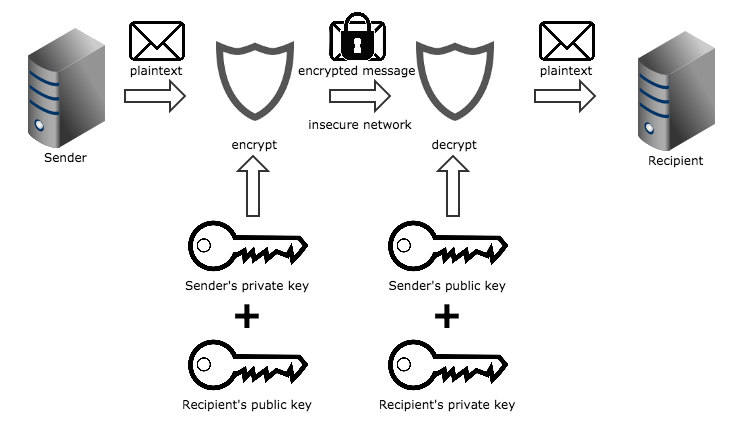
\includegraphics[width=0.8\textwidth]{paper-images/rsa-diagram.png}
\caption{}
\label{fig:rsa-diagram}
\end{figure}


\newpage
\section{Blockchain}

\subsection{Definition of a blockchain}

\iffalse
todo: 
- different interpretations of blockchain
- reread and remove weird references
\fi

In the last few years, the blockchain as a concept has been given a wide range in meanings and definitions: some explain the blockchain as a history of events, some focus on blockchain as a bitcoin transaction ledger and some talk about the open decentralized database aspect of blockchains \cite{blockchain-multiple-definitions}. Therefore, we will start out this paper by thoroughly defining this concept, to avoid any misunderstanding or confusion further on.

Antonopoulos (2014) \cite{antonopoulos:2014} defines the blockchain as follows: ``The blockchain data structure is an ordered, back-linked list of blocks and transactions.'' (p. 159). There are several aspects in this definition that need further explanation.

\subsubsection{Back-linked lists as data structure}

First of all, we are talking about a data structure: ``A specialized format for organizing and storing data'' \cite{data-structure}. There are several types of data structures such as arrays, lists, graphs, trees, etc.

Next, a blockchain is a specialized version of an ``ordered, back-linked list''. A list is data structure that combines a number of ordered values (Abelson 1996 \cite{abelson:1996}).  Incidentally, the ``ordered'' in the definition provided by Antonopoulos is superfluous, as by definition every list is ordered. An unordered list would no longer be a list, but would be a set instead. A blockchain will use back-linking to preserve the order of the values. This means that all values have a reference to the previous value in the list. For a blockchain, this means that every block in the blockchain contains an identification of the previous block. We will go further into hashes in a next section.

\subsubsection{Transactions}

Antonopoulos (2014) \cite{antonopoulos:2014} defines transactions as: ``data structures that encode the transfer of value between participants in the bitcoin system'' (p. 109). Although it gives a good idea of what transactions are, even in the context of the bitcoin blockchain this definition is complete: despite most transactions being value transactions between participants, a transaction can also store data on a blockchain. Even the bitcoin blockchain allows non-monetary transactions to be included.

Therefore, we can conclude that there are two types of transactions: monetary transactions and non-monetary transactions. In a monetary transaction, there is a transfer of value (eg. and amount of bitcoin) between participants. It must be noted that this does not have to be an instant transfer. Several blockchain protocols allow for a custom condition to be scripted into the transaction.

On the other side, there are non-monetary transactions that store data onto the blockchain. An example of a common used non-monetary transaction is the encoding of a document on the blockchain.

Transactions are the raison d'\^{e}tre of the blockchain. All aspects that we will discuss in this chapter exist to make sure that transactions can be validated, propagated over the network and added to a distributed ledger.

\subsubsection{Blocks}

Antonopoulos (2014) \cite{antonopoulos:2014} defines a block as: ``a container data structure that aggregates transactions for inclusion in the public ledger, the blockchain.'' (p. 160). A block is literally a wrapper for multiple transactions to make it possible for them to be included into the blockchain. These blocks then form the ordered values of the back-linked list addressed in the beginning of this section, each linking to the previous block in the list.

To conclude, the blockchain is a list of blocks, with each block containing several transactions.

\subsection{Properties of a blockchain}

\subsubsection{Securing the immutability of block headers}

\iffalse
- need to secure against attacks on the immutability of its blockchain. otherwise eg. considering a cryptocurrency system, an attacker could spend a coin and afterwards nullify this transaction by transmitting their own version of the blockchain without the spent transaction

- what are consensus mechansisms
\fi

As the Bitfury Group explains \cite{bitfury-pos-vs-pow}, every implementation of a blockchain must secure itself against possible attacks on its immutability. Take for example a blockchain powering a cryptocurrency. If the immutability of this blockchain was not ensured, an attack could spend a coin and afterwards transmit a version of the blockchain without this transaction. As a result, the attacker changed the blockchain to a new reality in which this coin has not been spent, allowing the attacker to spend this coin again.

To ensure this immutability, blockchains make use of a consensus mechanism, an algorithm the different entities in the network use to agree upon the newest state of the blockchain. Every consensus mechanism is designed in such a way that no one malicious entity can break the system unless this entity has some sort of majority in the network. How this majority is defined, depends on the consensus mechanism.

\iffalse
every consensus mechansism: 
- what is needed to suggest a new block
- how does this prevent 
- what are advantages and disadvantages
\fi

\paragraph{Proof of work}

\iffalse
- to suggest a new block, an entity needs to solve a random computational problem. This problem is designed as such that this entity, called the miner, has a chance of p% to solve this problem if he controls p% of the computing power currently in the network. If the miner solves the problem, he will be rewards with the relevant cryptocurrency. Consequently, miners are incentivised to provide as much computing power as possible until it is not longer economically interesting regarding the reward. 

- As the Bitfury Group correctly states \cite{bitfury-pos-vs-pow}: "[the] security of the network is supported by physically scarce resources: specialized hardware needed to run computations, and electricity spent to power the hardware." 
\fi

\iffalse
TODO: maybe add a small part about the alternative to a mining: merged mining and anchoring (cfr bitfury - group publc vs private prt 1)
\fi

To suggest a new block for a blockchain with a proof of work consensus mechanism, an entity needs to solve a random computational problem. This problem is designed as such that this entity, called the miner, has a chance of p\% to solve this problem if he controls p\% of the computing power currently in the network. If the miner solves the problem, the miner will be rewards with the relevant cryptocurrency. Consequently, miners are incentivized to provide as much computing power as possible until it is not longer economically interesting regarding the reward. As the Bitfury Group correctly states \cite{bitfury-pos-vs-pow}: "[the] security of the network is supported by physically scarce resources: specialized hardware needed to run computations, and electricity spent to power the hardware." (p.2)

If a malicious entity wants to manipulate a proof of work blockchain, this entity would need to control 50\% of the computing power on the network. Therefore, the security of a proof of work blockchain depends on two main factors. First is the total computing power in the network, also called the hash rate. A higher the hash rate means it is more difficult for a new entrant to suddenly take over the network. Second is the distribution of the computing power in the network. If a couple of entities hold a high percentage of the total computing power in the network, they could effectively work together achieve a majority share in the network.

The main advantage of a proof of work system is its security, as it is very costly to attack. However, this comes at a steep ecological cost as a lot of electricity and computing hardware is wasted on useless calculations. Therefore, other consensus mechanisms have been suggested.

\paragraph{Proof of stake}

The difficulty to create a new valid block for a blockchain with a proof of stake consensus mechanism will depend on the balance an entity holds of the relevant cryptocurrency. An entity with a higher balance will more easily find a valid block, without having to spend electricity and computing hardware required by the proof of work algorithm \cite{bitfury-pos-vs-pow}.

The main idea is that entities with a higher balance, are more invested in the currency and its success. If one entity would control more than 50\% of money available, it would be against his own interest to attack the blockchain as he would be hit the hardest. 

The advantage of this system is the absence of wasteful spending. Instead of having to spend \$1000 on specialized mining hardware, you can invest this money in the cryptocurrency itself with the same effect. However, there are several problems with the proof of stake mechanism. It is out of scope of this paper to discuss these issues individually, but all result out of the fact that the ``proof of stake consensus is not anchored in the physical world (cf. with hashing equipment in proof of work).'' (Bitfury Group, 2015, p22). 

The most valuable cryptocurrency using some variation of proof of stake mechanism is Bitshares, with a market capitalization of \$300 million on July 20, 2017 \cite{general-market-cap}, making it the 14th most valuable cryptocurrency at the time of writing. This shows how the market trusts the proof of work mechanism better. Furthermore, Bitshares' market capitalization was only \$20 million in April 2017 and reached a record of \$1.2 billion on June 10, 2017. This illustrates further the extreme volatility of cryptocurrencies.

\paragraph{Other consensus mechanisms}

Several other consensus mechanisms have been proposed, besides proof of work and proof of stake. An example is proof of storage, in which an entity will be able to create new blocks depending on how many megabytes of storage he can provide the network \cite{proof-of-whatever}. However, as most of these other consensus mechanisms have not been implemented in successful blockchains, it is very hard to evaluate their viability. 

\subsubsection{Access to the blockchain data}

As explained by the Bitfury Group \cite{bitfury-permissioned}, there are three levels of access to a blockchain. Firstly, there is read access to the data stored on the blockchain. This is the lowest level of access to a blockchain. Secondly, on a higher level, there is access to propose new transactions to the blockchain. Finally, on the highest level, there is access to create new blocks of transactions and add these blocks to the blockchain.

Depending on the design of a blockchain, different entities can have different levels of access to this blockchain.

\paragraph{Read access and and transaction submission: private and public blockchains}

The first two access levels are intertwined and will be discussed together.

As mentioned by the Bitfury Group \cite{bitfury-permissioned}, there are two options on these access levels. The first option is a public blockchain. This means that there are no restrictions an reading the data on the blockchain or on submitting transactions. The other option is a private blockchain. Only a predefined list of entities can then directly access the data or submit transactions.

Although a private blockchain might seem more secure because of the controlled access, the Bitfury Group \cite{bitfury-permissioned} shows that several of the advantages of using a blockchain are lost. First of all, several clients will not have direct access to the blockchain data, they will have to rely on a node with direct access. This works against the decentralized aspect of a blockchain as there are only a limited amount of possible nodes to connect to. Next, as clients need to connect to a node with full access, not only do they have to trust that node, the interaction with that node becomes a vulnerability as well. For example, a 'man in the middle attack' is possible. This means that when a user tries to interact with the blockchain, a malicious party could intercept this communication and reply with false information \cite{man-in-the-middle}. Finally, only a limited set of computers has access to the transactions on the blockchain, creating the possibility of a human factor intervening in the blockchain operation. This circumvents the reliance of the algorithmically enforced rules of a blockchain.

On the other hand, data on public blockchains can be properly encrypted. This will provide sufficient security and privacy in most use cases.

\paragraph{Access to transaction processing: permissioned and permissionless}

For the third level, the developer of the blockchain has to chose who is allowed to process transactions that get incorporated into the blockchain. The first option is a permissionless blockchain. On a permissionless blockchain, there are no restrictions on the identities of the transaction processors. The opposite is a permissioned blockchain. Only a predefined list of entities can process transactions. 

The use of a permissioned, public blockchain can be a necessary compromise in situations where compliance is an issue, such as in the financial sector.


\subsection{Examples of blockchains}

\subsubsection{Bitcoin}

% discuss: short introduction, properties, characteristics making it an interesting blockchain

The best known implementation of blockchain technology is in the bitcoin cryptocurrency. Bitcoin is a cryptocurrency created by Satoshi Nakamoto in 2008 \cite{bitcoin-paper}. In June 2017, bitcoin hit a record market capitalization of \$48.8 billion \cite{bitcoin-market-cap}. It is by far the most popular and best established cryptocurrency currently. The drawback of this popularity is the difficulty to change flaws in the system, resulting in crises such as the current block size crisis \cite{bitcoin-civil-war}.

The bitcoin blockchain is an public, permissionless blockchain with a proof of work consensus mechanism. This means that everyone has read access to the data on this blockchain, everyone can propose transactions to be added to the blockchain and everyone can start a node to help accepting proposed transactions.

The bitcoin blockchain uses a basic scripting language to power its transaction processing, only advanced enough to make a transactions and store short pieces of data \cite{antonopoulos:2014}. On one side, the simplicity of this language could be seen as a limitation of its potential. On the other hand, is it a feature of the bitcoin blockchain making it more secure.

The bitcoin blockchain is interesting because of its extreme security. In July 2017, the bitcoin blockchain mining network has a hash rate of around 6.6 exa hashes per second \cite{bitcoin-hash-rate}. This means that the bitcoin network is being supported by the equivalent computing power of 1.9 trillion Macbook Pro's from 2014. This shows the security of the bitcoin network. To break the system, one entity would need to suddenly control half of this computing power, which is quite unlikely. The only way would be to develop a supercomputer that is as a more powerful than all the computers ever made, such as a 50 qubits quantum computer \cite{quantum-newsweek}.

Because the bitcoin mining is so strong, it is often used by other cryptocurrencies and other blockchains to help secure their own network. Namecoin is such an example \cite{namecoin-whitepaper}.

\subsubsection{Ethereum}

Ethereum is another cryptocurrency powered by a blockchain, and the second most valuable cryptocurrency with a market capitalization of \$36.2 billion in June 2017. While bitcoin focuses on creating a secure, non-nonsense currency, ethereum tries to leverage the entire potential of the blockchain. This creates endless possibilities but makes ethereum also more complex than bitcoin.

Just like the bitcoin blockchain, the ethereum blockchain is currently public and permissionless with a proof of work consensus mechanism. However, there are plans to move to a proof of stake approach in the future \cite{ethereum-pos-faq}. 

As explained in the Ethereum white paper \cite{ethereum-whitepaper}, the programming language powering the ethereum blockchain, called Solidity, is Turing complete. Practically, this means that any conceivable program could be written in this language. This creates the possibility for smart contracts. These are transactions that will be executed automatically only if a certain condition is met. An example is a crowdfunding campaign that only transmits the raised budget to the beneficiary once the threshold is met before a certain deadline.

Because of its wide potential, the source code of the ethereum blockchain is often copied (called 'forked'), adjusted and redeployed for custom blockchain solutions. 


\newpage
\section{Distributed databases}
\label{sec:distributed-dbs}

\subsection{Distributed, decentralized and centralized databases}

\iffalse
- to fully comprehend distributed databases, we have to distinguish them from decentralized and centralized databases. baran 1964: in context of networks: distributed vs centralized and decentralized in between
- apply this definition to databases: add examples: one single database: standard example, decentralized: cloudfront CDN by amazon, distributed: bittorrent
\fi

To understand distributed databases, it is important to distinguish them from decentralized and centralized databases. Baran (1964) \cite{baran-distributed-communications} explains the difference in the context of networks. A centralized network makes all nodes connect to one central node. A distributed network is the opposite, in which any node can communicate with any other node without the need for a central node. Between lies the decentralized network, in which there are a couple of central nodes that communicate with each other. Other nodes have to connect with one of these central nodes.
Figure \ref{fig:baran-networks} visualizes the differences.

\begin{figure}[h]
\centering
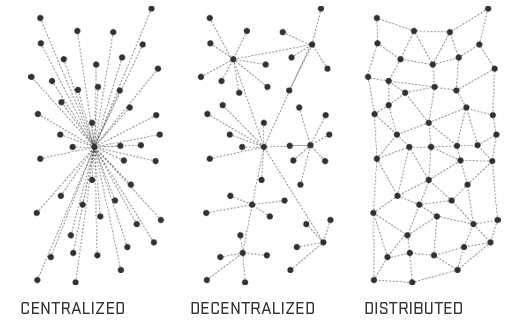
\includegraphics[width=0.8\textwidth]{paper-images/baran_networks.png}
\caption{Baran, P. (1964) Centralized, decentralized and distributed networks.} 
\label{fig:baran-networks}
\end{figure} 

This definition can be ported to the context of databases. A centralized database consists of one main data storage node. Users connect to this node to read and write data. A self-hosted website is a perfect example of a centralized database. Any user that wants to connect to your website, has to connect to your server. If your server breaks down, nobody can access the website anymore.

A decentralized database has many storage nodes that communicate with each other. A user can connect to either of these main nodes to access the data. Use of a CDN (Content Delivery Network) is an example of a decentralized database. Websites hosted on a CDN are copied across servers all over the world. To access to this website, a user can connect to any of these servers.

Finally, a distributed database does not have main storage nodes. Instead, every node can hold the entire database. When a new node wants to access the data, the node asks its peers for the data. Examples are BitTorrent and git, which both will be discussed further one in this chapter.

\subsection{Consistency, availability, and partition-resilience: the CAP theorem for distributed systems}

It is clear a trade-off is made when deciding between a centralized or distributed database. When a user reads data from a centralized node, the user receives the correct data, as there is only one version of the data. However, when this one centralized node somehow breaks down, nobody will be able to access the database anymore. Fox and Brewer (1999) \cite{brewers-theorem-paper} calls such a database not ``partition-resilient''. This means that when one node goes offline in the network, the system stops operating.

The opposite is true when working with a distributed database. Even though some nodes are offline, a user can always connect to the data through the other nodes. However, this comes at a drawback. The data the user reads is not necessarily the most updated version, as it could have been updated on another node in the meantime. Fox and Brewer (1999) calls such a database not ``consistent''.

To avoid the consistency issue, a distributed database can force all nodes to update to the most recent version before responding to anymore read requests. But it could happen that a connection between a not-updated node and the updated node is broken. This hinders the not-updated node in receiving the latest version of the data. The node will refuse any read requests until the connection is restored, to not provide incorrect information. This node is still online and functioning, but not responding to requests. Fox and Brewer (1999) calls such a database not ``available''.

The CAP theorem (Consistency, Availability, and Partition-resilience) states that any network can choose two out of three characteristics. The theorem was first proposed by Fox and Brewer (1999). It was formally proven by Gilbert and Lynch (2002) \cite{gilbert-lynch-cap-proof}.

\subsection{Issues with distributed databases in collaborative systems}
\label{subsec:issues-distributed-dbs}

In a guided system, there is one authoritative entity controlling every node in the network. But in a collaborative system, separate agents with individual incentives have to work together. This creates a whole new set of challenges, namely consensus and immutability issues.

Consensus issues arise when the database has been updated on two different nodes at the same time. Somehow, these two conflicting versions have to be merged. % For example, Alice spends a cryptocurrency coin to buy something from Bob. But at the same time, she uses this same coin to buy something from Claire. etc etc

Immutability issues emerge when the agreed upon the past can be changed. For example, Alice wants to spend a cryptocurrency coin. The merchant makes sure that the coin is valid and approves the purchase. But when immutability is not properly enforced, Alice can go into the database and manually remove the transaction. This nullifies the transaction, allowing Alice to spend the coin again. It is important to note that this idea of immutability is not related to the immutability representing the C in the CAP theorem.

\subsection{Examples of distributed databases and networks used in collaborative systems}
\label{subsec:examples-distributed-dbs}
% how does every example do on the CAP theorem, what are other disadvantages

This final part of the chapter discusses several common implementations of distributed databases and networks in the context of collaborative systems. 

\subsubsection{Git version control}

Git is the most popular distributed version control system. A version control system helps a developer to keep track of the changes he makes to his code. A distributed version control system helps developers collaborate on the same code base by keeping track of everyone's changes. Every developer has a version of the entire code base and all the changes ever made. While developing, a developer makes changes to his local code base. Once finished, he can publish his changes. Often, he publishes his work to a central computer with the latest code. Other developers will pull now and then the code from this central computer to update their local code base. A developer can also pull the code from a colleague, in case he wants to use specific changes that have not yet been added to the central code (Chacon \& Straub, 2014 \cite{git-manual-book}). This entire process is modeled in figure \ref{fig:distributed-vcs}.


\begin{figure}[h]
\centering
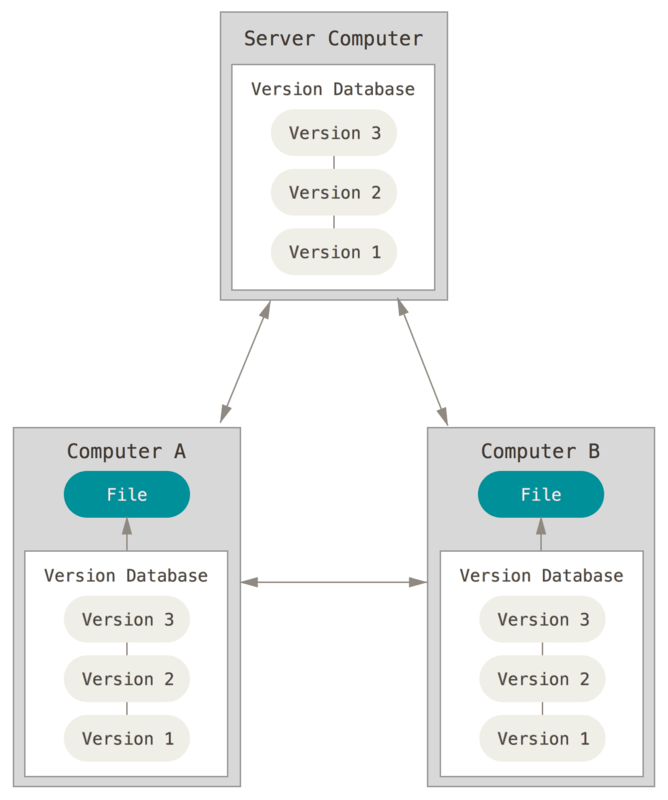
\includegraphics[width=0.4\textwidth]{paper-images/distributed.png}
\caption{Chacon \& Straub (2014) Distributed version control.} 
\label{fig:distributed-vcs}
\end{figure}

Git includes a specialized algorithm to automatically merge new changes into the code base. Consequentially, the consensus problem is often automatically solved. However, when two developers made changes to the same code, the algorithm fails, resulting in a ``merge conflict''. It is then up to the developer to manually solve the conflict. 

Immutability is not enforced in git. This means that any developer can manipulate the history of changes. This is useful when for example a large file has accidentally been included into the project. This bloats the size of the project and hampers collaboration. Simply removing the file does not help, as the file will still be part of the code history. To completely get rid of this file, the original inclusion has to be nullified. However, this could be used for malicious practices as well. Imagine a problem arises because of a programming mistake made some weeks ago. In case the developer does not want to be held accountable, he could remove his change from the history. Or he could even change the author of the change to someone else \cite{change-author-commit}.

It is clear that the git system needs trust between the developers. But in certain projects, there is no trust. For example, in open source projects, any developer can propose code changes. This is why on hosting sites for git repositories, such as Github, authorized users need to approve a code change before it can be added to the main code base \cite{github-pr}. But this partially removes the distributed character of git.

Considering the CAP theorem, it is clear git is available and partition-resilient, but not consistent. A node can always download a version of the code base, either from the main server or from one of its colleagues. This makes git available. If a node goes offline, a developer can contact any other developer for the full code base, making git partition-resilient. However, as every developer has a slightly different code base because of his own changes, git will never be consistent.

\subsubsection{BitTorrent}

BitTorrent is a peer-to-peer file distribution system. Instead of downloading a file from a central server, users download the file from peers that already (partially) have the file. However, once a file is uploaded with BitTorrent, it can no longer be changed. Most databases need some sort of write functionality. This characteristic disqualifies BitTorrent for most database applications. Yet, the single focus makes BitTorrent work really well for file sharing. As a result, BitTorrent was one of the first widely accepted collaborative, distributed networks. It ``increasingly becomes the norm for media acquisition among the general Internet public'' (Andersson, J. 2009 \cite{bittorrent-norm})

As there are no updates to a BitTorrent file, consensus and immutability are not an issue. Also, the CAP theorem is not relevant in this writeless context. BitTorrent is consistent, available and partition-resilient.

\subsubsection{Blockchain}
\label{subsubsec:blockchain-as-distributed-dbs}
\iffalse
- CAP Theorem
 => maybe add a section about database properties in general (CAP theorem) and the blockchain aspect of it (one of the papers mentions this, I think Bitfury)
- general advantages of blockchains as a database: consistency and consensus 
- disadvantages of blockchains: latency and scalability
\fi

The blockchain technology has already been explained in the previous section. Blockchain solves both the consensus issue as the immutability issue quite well. It is, therefore, a prime candidate for applications that require a collaborative database.

% consensus: forks and resolving
Blockchain handles the consensus issue quite well. As previously explained, once a miner has found a new valid block, he propagates this block through the blockchain network. Other miners will continue mining on the new block, as such appending the blockchain. But if two miners simultaneously find a valid block, they will both propagate this block through the network. Some miners will first receive one block and continue mining on top of that block, others will mine on top of the other block. In this case, there are effectively two different versions of the database. This phenomenon is called a fork. To solve this fork, miners are incentivized to work on top of the longest fork. As it is unlikely that miners will again simultaneously find a new valid block, one fork will quickly become longer than the other. This compels the miners to switch to the longest fork, thus resolving the fork \cite{antonopoulos:2014}. 

% TODO consistency: incredibly hard to rewrite history, as would need to recalculate all the blocks afterward

immutability is built into the blockchain idea. An attacker would first have to create a fork before a certain block he wants to alter. For this fork to be accepted as the proper blockchain, the attacker would need to make the fork longer than the current blockchain. Without more than 50\% of the network's computing power, this is mathematically impossible for blocks deep in the blockchain. As Nakamoto (2008) calculates in his paper, there is less than 0.1\% an attacker with 25\% of total computing power can catch up after 15 blocks have passed. As currently, the largest mining pool holds only 23.8\% \cite{hashrate-distribution}, waiting 15 blocks would be extremely safe. In general, the bitcoin community agrees that after 6 confirmation blocks a transaction is confirmed \cite{bitcoin-confirmation-amount}. For small transactions, best practice states that one confirmation block should suffice. Larger transactions might need three confirmation blocks \cite{confirmation-safety}.

% TODO cap: ap and eventually consistent: 

The CAP theorem can also be applied to blockchains. As Goland states in his blog \cite{blockchain-cap}, blockchains are available and partition-resilient and eventually consistent. As said before concerning the bitcoin blockchain, a user can be virtually sure that a block is immutable after 6 confirmation blocks \cite{bitcoin-confirmation-amount}.

However, there are some practical disadvantages with the blockchain. The first disadvantage is the lack of scalability of a blockchain. The main reason is that blockchain holds all transactions ever executed. As a result, the size of the blockchain constantly increases. This gradually pushes smaller nodes out of the network as they cannot afford to hold the entire blockchain in storage \cite{blockchain-scalability}. Another disadvantage is the latency of blockchains. To make sure a transaction has been included in the blockchain, merchants are expected to wait for some confirmation blocks. As the bitcoin blockchain for example creates one block every 10 minutes, this could be is an issue for several applications. Imagine going to a coffee shop and having to wait 30 minutes before you can get your coffee. Even though there are blockchains with lower block time (ethereum has a block time of 22 seconds \cite{ethereum-block-time}), these blockchains need more confirmations because of the higher chance of a fork. Finally, privacy could be an important concern on public blockchains. Although the data stored to the blockchain can be properly encrypted, everyone with read access to the blockchain can see when this data is submitted. Again, this could be a problem for certain applications.

\subsubsection{Non-persistent P2P networks}

The final aspect of this chapter discusses collaborative peer-to-peer (P2P) networks that are not persistent. This means that there the data on the network is not stored. It can only be accessed in real-time. 

An example of such a network is Open Bazaar. Open bazaar is a decentralized peer-to-peer marketplace. When a customer buys an item from eBay, the customer searches through listings that have been posted to the centralized servers of eBay. When searching for a specific item on Open Bazaar, a customer searches through the network of nodes that are currently online. But when a node posting a listing goes offline, this listing will no longer show up in search results \cite{openbazaar-faq}. This is why we call this a non-persistent network instead of a distributed database.

\iffalse
- no cap applicable, as not a database
- examples: open bazaar.
\fi


\newpage
\chapter{Aim of research}

\iffalse
- start with consensus and consistency in col. distr. dbs => because no central authority
- pivot into main idea: have technology replace an indispensable middleman. As discussed in \ref{subsec:examples-distributed-dbs}, blockchains solve both issues very well. 
- to apply the main idea to collaborative databases: two approaches. First a centralized collaborative database can be stored without a middleman. Second, the interaction between a nodes of a distributed collaborative database can be managed without a middleman
- For the first approach, the final chapter looks into proposals to store data in a distributed manner. Every proposal is examined on advantages, disadvantages, viability and current implementations.
- Concerning the second approach, the last chapter focuses on proposals to manage the interaction 
\fi

The central research question of this paper asks ``How can this idea to replace a middleman with technology be applied to collaborative, distributed databases?''. Section \ref{sec:distributed-dbs} shows collaborative, distributed databases face consistency and consensus issues. These issues arise because there is no central authority or trusted middleman. Sometimes some authority is created, such as in the example of git. However, section \ref{subsubsec:blockchain-as-distributed-dbs} indicates that blockchain solves both the consensus and consistency issue without the need for a trusted authority.

When applying the main idea of replacing a middleman with technology to collaborative databases, two use cases come up. The first case focuses on a centralized database that is stored without a trusted middleman. The second case examines the management of the interactions between the nodes of a distributed database without a central, guiding authority.

The first case studies centralized, collaborative databases. Centralized databases have not been heavily covered in the previous chapters as they are rather trivial. But it is, of course, possible to collaborative on a centralized database as well. An example would be a shared Dropbox folder. Several users work together on the same files, stored at a trusted third party \cite{dropbox-sharing}. The final chapter looks into proposals to store this data in a distributed way instead. It is important to note that proposals in this category do not intent to solve either consensus or consistency issue. Because the collaborative databases are centralized to begin with, this would not be possible.

The second case focuses on decentralized, collaborative databases. As often discussed before, the two main issues are consensus between the nodes and consistency between the data stored on the nodes. The final chapter examines several proposals to manage these interactions in a distributed manner without a central authority.



\chapter{Proposed solutions}

\section{Storing centralized data onto a blockchain}
\label{store-on-Bitcoin}

\iffalse
- very obvious solution would be to store data directly onto a blockchain, eg. the Bitcoin blockchain. you would just put all the data, properly encrypted, directly onto the blockchain and it is stored

\fi

An obvious proposal is to store centralized data directly onto a blockchain, for example onto the Bitcoin blockchain. A user could encrypt his data and store it onto the Bitcoin blockchain using a data transaction. Anyone else with the proper key could access this data and submit an updated version.

\iffalse
- various issues arise: 
  - basic functionality is missing that several applications need: you are not able to change or remove data once stored data, to update a file you would have to store the entire file again or store just the change and have your application reading the blockchain create the most recent file.
  - as mentioned in section \ref{subsubsec:blockchain-as-distributed-dbs}, blockchains deal with low scalability, high latency and potential privacy concerns.
  - insanely expensive: 0.0000026 BTC per byte \cite{Bitcoin-transaction-fee}. At a current market cap of €2418.09 per BTC, the cost of storage is €6.44 per KB. \cite{Bitcoin-market-cap}
\fi

However, there are multiple issues with this approach. 

First, it is not possible to change or remove data once it is stored onto the blockchain. To update a file, the user would have to upload the entire new file. Another option is to store just the changes to the original file onto the blockchain. In this case, the application used to read the data from the blockchain would create the most recent version of the file based on the original file and the submitted changes. 

Secondly, blockchains' characteristics such as low scalability, high latency, and potential privacy concerns make them useless for most centralized database applications. These issues have been thoroughly discussed in section \ref{subsubsec:blockchain-as-distributed-dbs}.

Finally, storing data onto a blockchain is very expensive because of its low scalability. Considering the Bitcoin blockchain, every byte of storage costs 0.0000026 BTC \cite{Bitcoin-transaction-fee}. At a current market cap of \euro 2418.09 per BTC, 1 KB costs \euro 6.44 \cite{Bitcoin-market-cap}.

\iffalse
- because in a context of centralized database, immutability and consensus as are not issues. Solving these problems is the main selling point of blockchain. Although it might be interesting that blockchain provides immutability, this could also be a problem. Some centralized databases might require delete functionality. This is no possible when using a blockchain

- not viable for storage of normal amounts of data
\fi

On the other hand, the main selling point of using a blockchain is solving the immutability and consensus issues. But these are not seen as issues in a context of centralized databases. On the contrary, enforced immutability could be a problem for certain applications that require delete functionality.

Because of these reasons, it is clear that blockchains are not a viable instrument to store normal amounts of centralized data directly.
\newpage
\section{Distributed cloud storage}
\label{blockchain-distributed-storage}

\iffalse

- idea: instead of trusting a central party: 
  - divide your storage data into little pieces and send the pieces to different storage providers => process of dividing is referred to as sharding. storage providers can be anyone: large companies with data centers or individuals with available space on their hard drive. 
  - you send your shards of data to a storage provider. you can send every shard just once, or you could store it multiple times to be sure your data never disappears. the renter pays the hosts for the time they store their data.

- however: multiple issues arise in this system: what if a host promises to store your data, but actually does not, what if a renter doesn't pay for the used storage space?

- there are currently several solutions out there that try implement this concept, such as siacoin, storj and swarm. Others, such as ipfs and maidsafe, want to go even further trying to replace the internet as we know it.

\fi

A distributed cloud storage network replaces a trusted storage provider such as Amazon or Dropbox with a large network of storage providers. Storage providers can be large companies with data centers to their disposal or individuals with free storage space on their hard drive. These storage providers are referred to as the hosts. 

When a user, called a renter, wants to store his data on the network, he divides his data into small pieces. The renter then sends these pieces to the hosts. For extra redundancy and security, the renter duplicates his pieces several times on the network. The renter then pays the hosts for the time they store their data.

This simple concept faces multiple issues. A host could promise to store a renter's data without actually keeping the data. A renter would have to do some insane redundancy duplication on the network to safely store his data, while still being at risk of losing an essential piece. On the other hand, a host storing a renter's data is never guaranteed the renter will actually pay.

Currently, several solutions try to implement this concept. Siacoin \cite{siacoin} and Storj \cite{storj} focus on cloud storage. Others, such as IPFS \cite{IPFS} and Maidsafe \cite{maidsafe}, want to go further and are trying to replace the internet as it currently works. This thesis will focus on cloud storage and compare two current commercial solutions: Siacoin and Storj.


\subsection{Storj}

\iffalse
# storj

- storj: uses a pay as you go system. every now and then you ask your storage providers for a proof that they are still holding your data. if you receive this proof, you pay them. If you do not receive a proof, you can assume this data is lost and make sure that piece of your date is reduplicated on the network. if a storage provider does not get paid for his proof, he can assume the user does not longer require him to store the data allowing him to delete this shard. 

- There are still some issues though: 
  - hosts take a risk when storing data, as they are never sure they will be paid. in the most extreme case, a malicious host might store a lot of data on the network, but never pay the first proof of storage, wasting this storage space. This effectively executes a denial of service attack on the network.
  - hosts do have no cost of not providing a proof of storage. 
  this makes the network very vulnerable to a sybil attack \ref{sybil-attack}. in which one malicious agent pretends to be several hosts at same time, at no cost. renters might think their data is secure, as it is duplicated over several hosts. However, the one malicious agent can turn off all his hosts, effectively destroying the stored data.


\fi


Storj uses a pay as you go system. From time to time, the renter asks the hosts for a proof of storage that they still hold the data. If the renter receives this proof, he pays them. If the renter does not receive the proof, his assumes this host does no longer store his data and the renter makes sure that piece is reduplicated on the network. If a host does not receive a payment for a proof of storage, he assumes the renter does no longer require him to store the data and that he can delete the renter's data. \cite{storj}

Although this solves some of the original incentive issues, there are still other issues. 

Hosts are never sure they will be paid when storing data. This means that the network is vulnerable to a denial of service attack. If a malicious agent stores a lot of data on the network without ever paying the first proof of storage, the network's storage space is being wasted, making it unavailable for honest renters.

Furthermore, hosts still have no cost of not providing a proof of storage. This makes the network more vulnerable to a Sybil attack \cite{sybil-attack}, in which a malicious agent pretends to be multiple hosts without any cost. A renter might think his data is secure as it seems duplicated over several hosts. However, the malicious agent controlling these hosts could destroy the data at any time.

\subsection{Siacoin}

\iffalse
#siacoin

- instead of pay as you go system, uses siacoin a blockchain to support their storage network. A host and a renter both sign a smart contract onto the siacoin blockchain. In this smart contract, the renter puts in his payment for the storage and the host puts in a collatoral in case he is not able to produce a proof of storage when the contract expires. Consequentially, the host is assured he will be paid by the blockchain, even when the renter is offline at the time the contract expires. And the renter is has a better assurance the host will provide the stored data as he would be rewarded the collatoral instead.

- Because the siacoin blockchain is publicly available, hosts' peformance is publicly visible. Hosts that are always providing a proof of storage when asked will be very reputable, while hosts that are less available will have a lower reputation or might even be blacklisted.
gs
- Finally, siacoin has an additional protection against a sybil attack. Although hosts have to pay a collateral if they do not provide a proof of storage, a malicious agent might still spin up an insane amount of hosts. His hosts are very likely to be picked to store data for the same renter. While it is not costless, the data duplication redundancy is not sufficient to prevent the malicious agent from effectively destroying the data of this renter. To prevent this situation, renters expect hosts to prove they are real by providing a proof-of-burn. This means that a host send coins to an address that cannot spend these coins.

\fi

Instead of a pay as you go system, Siacoin uses a blockchain to support their network. A host and a renter both sign a smart contract onto the Siacoin blockchain. In this smart contract, the renter puts in his payment for the storage and the host puts in a collateral in case he is not able to produce a proof of storage when the contract expires. Consequentially, the host is assured he will be paid by the blockchain, even when the renter is offline at the time the contract expires. The renter has a better assurance the host will provide the stored data as he would be rewarded the collateral instead.

Because the Siacoin blockchain is publicly available, hosts' performance is publicly visible. Hosts that always provide a proof of storage when asked, will be very reputable. Less available hosts will have a lower reputation or might even be blacklisted.

Finally, Siacoin has an additional protection against a Sybil attack. Although hosts have to pay a collateral if they do not provide a proof of storage, a malicious agent might still spin up an insane amount of hosts. His hosts are very likely to be picked to store data for the same renter. While it is not costless, the data duplication redundancy is not sufficient to prevent the malicious agent from effectively destroying the data of this renter. To prevent this situation, a renter expects a host to prove they are real by providing a proof-of-burn. This means that a host sends coins to an address that cannot spend these coins. \cite{siacoin}
\newpage
\section{Timestamping a database}
\newpage
\section{Applied example: replacing notary testament services}
\label{notary-will}

\iffalse
- this section will discuss the role of a notary in writing a testament and how this can be replaced by technology. The notary can be seen a trusted storage provider for centralized storage, the testament.

- It is not necessary by Belgian law to have a notary witness or store a testament \cite{eigen-testament}. However, they are still often used to witness the signature, store the testament and in general make sure everything is correct. This section will show a notary's service can be fully replaced by public key encryption, a blockchain and a regular lawyer, as the main difference between a regular lawyer and a notary is a notary's ability to witness a signature. The section starts with a very simple solution, but will gradually expand the proposal to make sure that by the end all aspects of a notary's testament service is covered.
\fi

This section will discuss how a notary's testament service can be replaced by technology. In the context of centralized databases, the notary can be seen a trusted storage provider for centralized storage, the testament.

It is not necessary by Belgian law to have a notary witness or store a testament for the testament to be valid \cite{eigen-testament}. However, notaries are often used to witness the signature, store the testament and in general make sure everything is correct. This section will show how a notary's service can be fully replaced by public key encryption, a blockchain and a regular lawyer with no authority concerning witnessing signatures. The section starts with a very simple solution. The proposal will be gradually expanded, so all aspects of a notary's testament service are covered.

\iffalse
- signature. As mentioned before, the main reason for a notary's service is his witnessing of the signature. Because a testament can be a valuable document, several different parties might be incentivised to falsify the document and the signature. As the testator will be deceased, he will not be able to testify in court. 

- with the incorporation of the digital signature into every Belgian ID, every Belgian has the possibility to sign any document digitally (D. De Win, personal communication, July 19, 2017). A digital signature is more secure than a manual signature, as it cannot be faked or immitated \cite{belgian-eid}.

- in the simplest example, a testator writes his testament with the help of a regular lawyer to make sure all wording is correct. He then signs a digital version with his digital signature. Finally, he distributes the signed document to all potential stakeholders: family, friends, beneficiary institutions. He could even publish his signed testament online to make sure any stakeholder could access it.
\fi

\subsection{Signature}

 As mentioned before, the main reason for a notary's service is the witnessing of the signature. Because a testament can be a valuable document, several parties might be incentivized to falsify the document and the signature. As the testator will be deceased, he will not be able to testify in court to verify his signature.

 With the incorporation of the digital signature into every Belgian ID, every Belgian has the possibility to sign any document digitally (D. De Win, personal communication, July 19, 2017). A digital signature is more secure than a manual signature, as it cannot be faked or imitated \cite{belgian-eid}. 

 In the simplest solution, a testator writes his testament with the help of a regular lawyer to make sure all wording is correct. He then signs a digital version with his digital signature. Finally, he distributes the signed document to all potential stakeholders: family, friends, beneficiary institutions and other recipients. He could even publish his signed testament online to make sure every stakeholder could access it.


\subsection{Extra security with a blockchain}

\iffalse
- blockchain

- A malicious agent could try to steal the testator's ID in the hours after the testator's death. If this agent knows the pin code of the testator's ID, he could forge a fake testament.

- to avoid this situation, the testator could store a fingerprint of the signed testament onto a public blockchain, eg. the bitcoin blockchain. In this situation, it is proven that a document had to exist before the fingerprint had been incorporated into the public blockchain. Because of blockchains' consistency, it would be impossible to fake this.

- storing a fingerprint onto a public blockchain has another advantage as well. it is no longer necessary to date the testament, as the earliest fingerprint on the blockchain can be seen as the date of creation.
\fi

In this simple proposal, a malicious agent could try to steal the testator's ID in the hours after the testator's death. If this agent knows the pin code of the testator's ID, he could forge a fake testament.

To avoid this situation, the testator could store a fingerprint of the signed testament onto a public blockchain, eg. the bitcoin blockchain. In this situation, it is quickly proven that a document had to exist before the fingerprint had been incorporated into the public blockchain. 

Storing a fingerprint onto a public blockchain has another advantage as well. It is now no longer necessary to date the testament, as the earliest fingerprint on the blockchain can be seen as the date of creation.

\subsection{Secret keeping}

\iffalse
secret keeping

- The final aspect of a notary's testament service that has not yet been covered by the blockchain alternative is secret keeping. In general, a notary will only reveal the contents of a testament once the testator is deceased. The current blockchain alternative is expecting the testator to distribute his testament to all stakeholders before he dies. This could result in some uncomfortable conversations.

- An ethereum script could solve this final aspect. Instead of distributing the testament, the testator could distribute an encrypted version of the testament instead. He could then store the key to decrypt the testament into a script on the ethereum blockchain. This script would only release the decryption key once the testator has deceased. There are several ways for this script to determine whether the testator is effectively deceased. For example, the testator could distribute keys to family and friends. These keyholders can then vote to release the decryption key, with the testator a veto. Another solution could routinely ask a public governmental database whether the testator has been declared deceased.
\fi

The final aspect of a notary's testament service that has not yet been covered by the blockchain alternative is secret keeping. A notary will only reveal the contents of a testament once the testator is deceased. The current blockchain alternative is expecting the testator to distribute his testament to all stakeholders before he dies. This could result in uncomfortable, unwanted conversations.

An ethereum script could solve this final aspect. Instead of distributing the testament, the testator could distribute an encrypted version of the testament instead. He could then store the key to decrypt the testament into a script on the ethereum blockchain. This script would only release the decryption key once the testator has deceased. There are several ways for this script to determine whether the testator is effectively deceased. 

There are several approaches to write this script. The testator could distribute keys to family and friends. These key holders can then vote to release the decryption key, with the testator given a veto. If the testator is not yet deceased, he will always be able to block the release the key. The rationale of using a voting system is to prevent immediate publication if the testator is offline for a while and unable to exercise his veto. Another solution could involve a script that routinely asks a public governmental database whether the testator has been declared deceased.

\newpage
\chapter{Conclusion}

%  BIBLIOGRAPHY
\begin{thebibliography}{99}\addcontentsline{toc}{chapter}{Bibliography}

\bibliographystyle{plain}

\bibitem{antonopoulos:2014}
{\sc Antonopoulos, A. M.} (2014).
Mastering Bitcoin.
{\em} Sebastopol, CA.

\bibitem{ceasar-cypher}
Cipher, C., \& Cipher, M. (2004). Introduction to cryptography. EEC, 484, 584.

\bibitem{rsa-patent}
Rivest, R.L. and Shamir, A. and Adleman, L.M. US Patent 4,405,829 issued in 1983

\bibitem{rsa-paper-explanation}
Calderbank, M. (2007). The RSA Cryptosystem: History, Algorithm, Primes.

\bibitem{data-structure}
{\sc data structure} (February 2006). Retrieved 23rd March 2017, from http://searchsqlserver.techtarget.com/definition/data-structure.

\bibitem{abelson:1996}
{\sc Abelson, H. et al.} (1996).
Structure and Interpretation of Computer Programs.
MIT Press.

\end{thebibliography}


\vfill

\appendix
\tocless \chapter{}
\addcontentsline{toc}{chapter}{Appendix}
\section{Appendix}


\newpage
\thispagestyle{empty}
\newgeometry{textwidth=540pt,textheight=780pt,top=20pt,left=20pt,right=20pt}
\begin{figure}[ht]
\begin{flushright}

\includegraphics[width=0.5\textwidth,natwidth=310,natheight=10]{./template_images/Picture3.png}
\end{flushright}
\end{figure}
\vfill
\begin{picture}(550,40)
\put(0,0){\colorbox{kuleuven}{\makebox(520,52){}}}
\end{picture}
\end{document}
